\documentclass{article}
\usepackage[utf8]{inputenc}
 \usepackage{amsmath}
 \usepackage{amssymb}
 \usepackage{graphicx}

 \newcommand\xk{\mathbf{x}^{\left(k\right)}}
  \newcommand\xkn{\mathbf{x}^{\left(k + 1\right)}}
    \newcommand\xko{\mathbf{x}^{\left(k - 1\right)}}
  \newcommand\xnNorm{\left\lVert\mathbf{x}^{\left(k + 1\right)} - \mathbf{x}^{\left(k\right)} \right\rVert}
  
  \newcommand\xoNorm{\left\lVert\mathbf{x}^{\left(k\right)} - \mathbf{x}^{\left(k-1\right)} \right\rVert}
  
  \newcommand\xsNorm{\left\lVert\mathbf{x}^{\left(k + 1\right)} - \mathbf{x}^{*} \right\rVert}
 
\begin{document}
\section*{Aspects of Iterative Methods for Non-Linear Equations}
\subsection*{8-17.a}
A \textbf{convergent} sequence $\xk\, , \: k = 0,1,2, \dots$ in $\mathbb{R}^{n}$ with limit $\mathbf{x}^{*}$ converges with \textbf{order} p, $p \geq 1$, if
\begin{equation*}
    \exists\,C >0 \: : \: \xsNorm \leq C \xnNorm^{p} \quad \forall \: k \in \mathbb{N}_{0}
\end{equation*}
and, in addition $C < 1$ in the case of p = 1. Do not forget the power $p$ as this is what makes it a convergence of \textbf{order} p.
\subsection*{8-17.b}
The code segment below is given to us.
\begin{figure}[!hbt]
    \centering
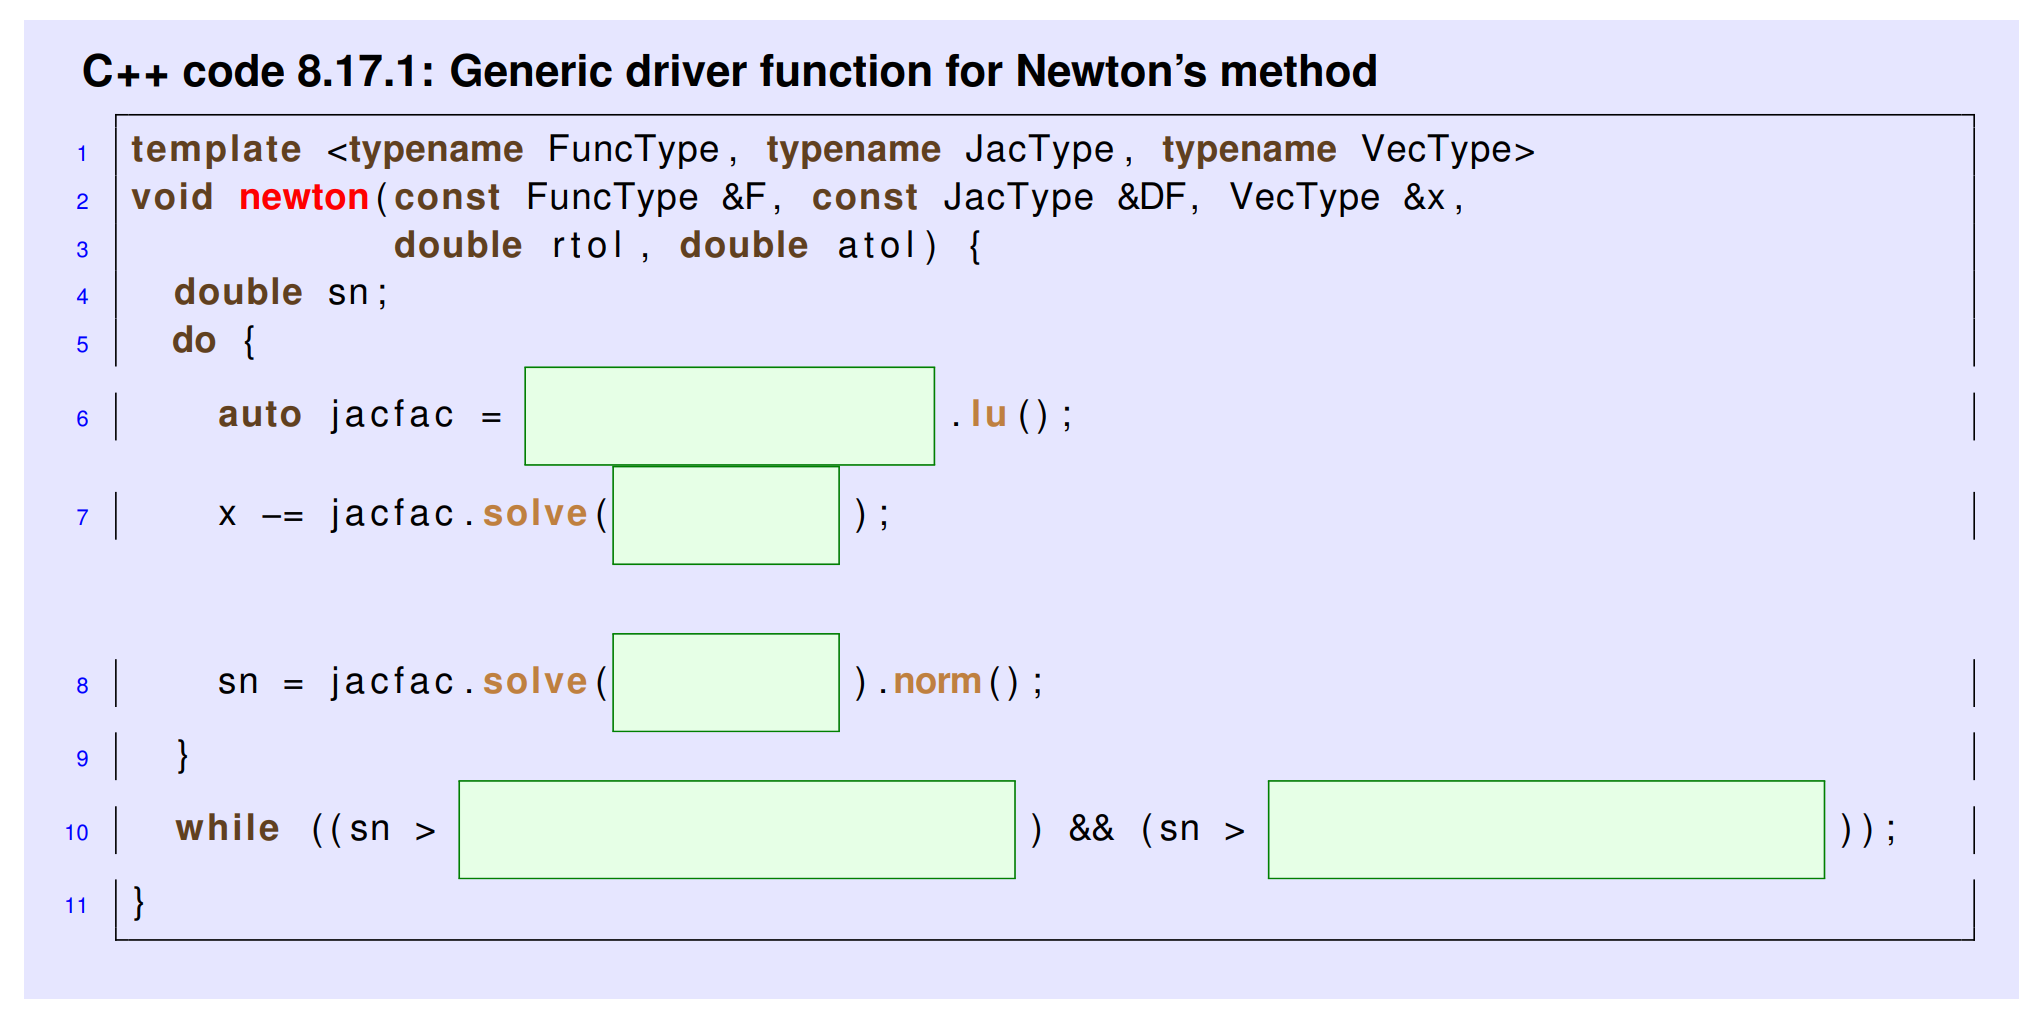
\includegraphics[width=1.1\linewidth]{CodeSegment.png}
\end{figure}
It implements a generic Newton iteration for solving $F\left(\mathbf{x}\right) = \mathbf{0}$, with correction-based termination relying on the simplified Newton correction.
\begin{figure}[!hbt]
    \centering
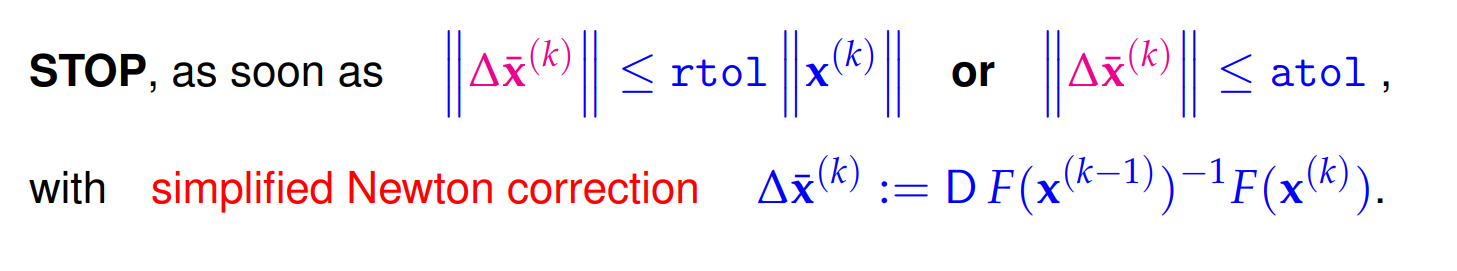
\includegraphics[width=0.7\linewidth]{NewtonIterationGeneric.png}
\end{figure}
The parameter \textit{x} supplies the initial guess, the functor \textit{F} represents the function, the functor \textit{DF} represents the derivative of the function, the parameter \textit{x} is also used to return the final result. 

\pagebreak

\noindent Seeing as the the Newton Iteration is given to us by
\begin{equation*}
\mathrm{D}F\left(\xko\right)^{-1}F\left(\xk\right)
\end{equation*}
we use an idea from an other exercise again. We could solve the system
\begin{equation*}
    \mathrm{D}F\left(\xko\right)\mathbf{y} =F\left(\xk\right) 
\end{equation*}
for $\mathbf{y}$ ($\mathbf{y}$ is just some placeholder variable) and get
\begin{equation*}
    \mathbf{y} = \mathrm{D}F\left(\xko\right)^{-1}F\left(\xk\right)
\end{equation*}
In code this would translate to the following lines. $\\[2mm]$
\noindent \verb|auto jacfac = DF(x).lu();| $\newline$
\noindent \verb|x -= jacfac.solve(F(x));| $\\[2mm]$
Remembering that the the simplified Newton correction is based on checking for
\begin{equation*}
    \xnNorm = \left\lVert \mathrm{D}F\left(\xk\right)^{-1}F\left(\xk\right)\right\rVert < \tau \left\lVert \xk\right\rVert
\end{equation*}
We can see that we have just computed the left side term. We have also seen that this is uneconomical and that if the methods terminates based on this correction $\xk$ would have already been accurate enough. We have also seen that because of the fast asymptotic quadratic convergence, we can expect $\mathrm{D}F\left(\xko\right) \approx \mathrm{D}F\left(\xk\right)$ and hence we can now check if
\begin{equation*}
    \xoNorm \approx \left\lVert \mathrm{D}F\left(\xk\right)^{-1}F\left(\xk\right)\right\rVert < \tau \left\lVert \xk\right\rVert
\end{equation*}
and the middle term is exactly what we compute in the next line $\\[2mm]$
\verb|sn = jacfac.solve(F(x)).norm();| $\\[1mm]$
Keep in mind that the \textit{x} here does not refer to the same \textit{x} as in the lines before, as it is the next iterate already. We hence have
\begin{equation*}
    \text{sn} = \left\lVert \mathrm{D}F\left(\xk\right)^{-1}F\left(\xk\right)\right\rVert = \left\lVert \Delta \tilde{\mathbf{x}}^{\left(k\right)}\right\rVert
\end{equation*}
and can do the following tolerance comparisons. 
\begin{equation*}
    \text{sn} \leq \text{rtol} \left\lVert \xk\right\rVert \quad \text{\textbf{or}} \quad  \text{sn} \leq \text{atol}
\end{equation*}
Which gives us the last two lines, where here we used so simple Boolean logic to check to negations with and instead of just or. $\\[2mm]$
\verb|(sn > rtol * x.norm()) && (sn > atol)|

\pagebreak

\noindent Together this gives us the code
\begin{figure}[!hbt]
    \centering
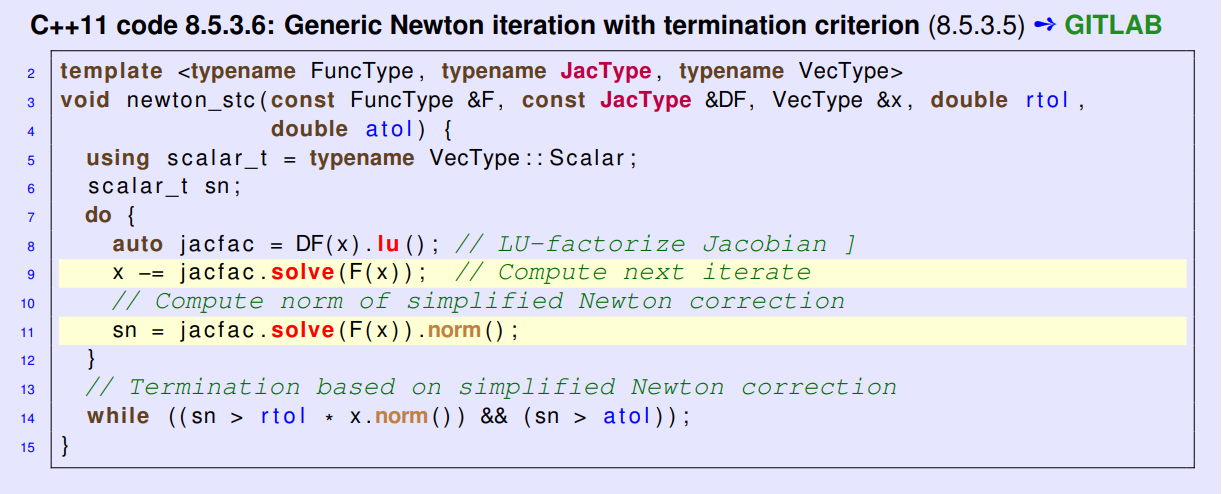
\includegraphics[width=1.2\linewidth]{8-17.b.png}
\end{figure}
\subsection*{8-17.c}
Let $f$ denote the function
\begin{equation*}
    f : \begin{cases}
        \left[0,1\right] \to \left[0,1\right] \\
        \hspace{6px} x \hspace{8px} \mapsto xe^{x-1}
    \end{cases}
\end{equation*}
We are tasked with stating the \textbf{Newton iteration} converging to $g\left(y\right)$ for a give $y \in \left[0,1\right]$ and sufficiently good initial guess $x^{\left(0\right)}$, where $g:=f^{-1}$ is the \textbf{inverse function} of $f$. The important part here is to recognise that finding the inverse is not really an option here as most tricks I have tried do not work. We know that $f\left(g\left(y\right)\right)$ and hence we want to find a $x$ for which 
\begin{equation*}
    f\left(x\right) = y \Longleftrightarrow f\left(x\right) - y = 0
\end{equation*}
We hence have found our iteration function in
\begin{equation*}
    F\left(x\right) = f\left(x\right) - y 
\end{equation*}
and we want to solve for $F\left(x\right) = 0$. The derivative (where $y$ is a constant) is given by
\begin{equation*}
    F'\left(x\right) = f'\left(x\right) = e^{x-1} + xe^{x-1} = \left(x + 1\right)e^{x-1}
\end{equation*}
The Newton iteration is as always given to us by
\begin{equation*}
    x^{\left(k+1\right)} = x^{\left(k\right)} - \frac{F\left(x^{\left(k\right)}\right)}{F'\left(x^{\left(k\right)}\right)}
\end{equation*}
We must verify that $F'\left(x^{\left(k\right)}\right) \neq 0$, but for $x \in \left[0,1\right]$ we have that $\left(x+1\right)e^{x-1} > 0$ and hence this is not  a problem. This gives us the final Newton Iteration
\begin{equation*}
    x^{\left(k+1\right)} = x^{\left(k\right)} - \frac{x^{\left(k\right)}e^{x^{\left(k\right)}-1}-y}{\left(x^{\left(k\right)} + 1\right)e^{x^{\left(k\right)}-1}}\,,\quad k \geq 0
\end{equation*}

\end{document}
